\documentclass[11pt,a4paper]{article}

\usepackage{fontspec}
\usepackage[utf8]{inputenc}
\usepackage[T1]{fontenc}
\usepackage[brazilian]{babel}
\usepackage[left=2.5cm,right=2.2cm,top=2.3cm,bottom=2.2cm]{geometry}
\usepackage{mathptmx}
\usepackage{setspace}
\usepackage{microtype}
\usepackage{enumitem}
\usepackage{graphicx}
\usepackage{titlesec}
\usepackage{array}
\usepackage{longtable}
\usepackage{xcolor}
\usepackage{fancyhdr}
\usepackage{tikz}
\usepackage[skins]{tcolorbox}
\usetikzlibrary{positioning,arrows.meta}
\newcolumntype{L}[1]{>{\raggedright\arraybackslash}p{#1}}

% ---------- paleta (a mesma dos diagramas do projeto) ----------
\definecolor{azul}{RGB}{31,73,125}
\definecolor{verde}{RGB}{27,127,92}
\definecolor{laranja}{RGB}{178,106,0}
\definecolor{vermelho}{RGB}{192,57,43}
\definecolor{cinza}{RGB}{82,96,109}

\titleformat{\section}{\normalfont\large\bfseries\color{azul}}{\thesection}{1em}{\MakeUppercase}
\titlespacing*{\section}{0pt}{14pt}{6pt}
\titleformat{\subsection}{\normalfont\normalsize\bfseries\color{azul}}{\thesubsection}{1em}{}
\titlespacing*{\subsection}{0pt}{8pt}{4pt}
\setlist{itemsep=2pt,topsep=3pt,leftmargin=1.3em}
\setstretch{1.04}
\emergencystretch=4em

\pagestyle{fancy}
\fancyhf{}
\renewcommand{\headrulewidth}{0pt}
\fancyfoot[L]{\footnotesize\color{cinza}Roteiro de prática: HC-SR04 nos nós N01 e N02}
\fancyfoot[R]{\footnotesize\color{cinza}Página \thepage}

\newfontfamily\codfont{DejaVu Sans Mono}[Scale=0.86]
\newcommand{\cod}[1]{{\codfont\hyphenchar\font=-1 \frenchspacing\detokenize{#1}}}
% linha de log do firmware (começa com "# ")
\newcommand{\logl}[1]{{\codfont\hyphenchar\font=-1 \frenchspacing\char35~\detokenize{#1}}}
\newcommand{\caixa}{\fbox{\rule{0pt}{1.6ex}\hspace{1.6ex}}}

% ---------- caixas de destaque ----------
\newtcolorbox{atencao}{enhanced,colback=vermelho!6,colframe=vermelho,boxrule=0.6pt,arc=2pt,
  left=7pt,right=7pt,top=5pt,bottom=5pt,
  title={\textbf{ATENÇÃO}},fonttitle=\sffamily\small,coltitle=white,colbacktitle=vermelho}
\newtcolorbox{dica}{enhanced,colback=azul!5,colframe=azul,boxrule=0.6pt,arc=2pt,
  left=7pt,right=7pt,top=5pt,bottom=5pt,
  title={\textbf{DICA}},fonttitle=\sffamily\small,coltitle=white,colbacktitle=azul}

% \passo{numero}{titulo}{tempo}{o que fazer}{resultado esperado}{onde ver}
\newcommand{\passo}[6]{%
\begin{tcolorbox}[enhanced,colback=white,colframe=azul,boxrule=0.6pt,arc=2pt,
  left=8pt,right=8pt,top=5pt,bottom=5pt,before skip=7pt,after skip=7pt,
  title={\textbf{PASSO #1} \enspace #2 \hfill {\small #3}},
  fonttitle=\sffamily\bfseries\small,coltitle=white,colbacktitle=azul]
{\sffamily\bfseries\small\color{azul}O QUE FAZER}\par\vspace{2pt}
#4\par
\vspace{5pt}
\begin{tcolorbox}[enhanced,colback=verde!8,colframe=verde,boxrule=0.5pt,arc=1.5pt,
  left=6pt,right=6pt,top=3pt,bottom=3pt]
{\sffamily\bfseries\small\color{verde}RESULTADO ESPERADO}\par\vspace{2pt}
#5\par
\end{tcolorbox}
\vspace{3pt}
{\sffamily\bfseries\small\color{cinza}ONDE VER:} #6
\end{tcolorbox}}

\newcommand{\fase}[2]{%
\vspace{6pt}
\noindent\begin{tikzpicture}
  \node[fill=#1,text=white,rounded corners=2pt,inner xsep=8pt,inner ysep=3pt,font=\sffamily\bfseries\small] {#2};
\end{tikzpicture}\par\nopagebreak}

\begin{document}

\begin{center}

\includegraphics[height=1.8cm]{../assets/ufc_logo.png}\par
\vspace{0.2cm}
{\normalsize UNIVERSIDADE FEDERAL DO CEARÁ -- UFC\par}
{\normalsize CENTRO DE TECNOLOGIA\par}
{\normalsize CURSO DE ENGENHARIA DE COMPUTAÇÃO\par}
\vspace{0.5cm}
{\Large \textbf{ROTEIRO DE PRÁTICA:\\ MONTAGEM E TESTE DO SENSOR HC-SR04}\par}
\vspace{0.2cm}
{\large Nós N01 (gateway e máquina 1) e N02 (sensor remoto, máquina 2)\par}
\vspace{0.4cm}
{\small
Antonio Marcos Justino Carneiro \quad João Victor Leandro Nunes \quad João Lucas Oliveira Mota\par
Anderson Moura Costa do Nascimento \quad Álvaro Siqueira Galvão\par
Disciplina de Sistemas Embarcados (TI0148) -- 2026.2 \quad Professor: Dário Queiroz\par
Fortaleza, CE -- quinta-feira, 26 de novembro de 2026 (laboratório)\par}
\end{center}

% =========================================================
\section{Objetivo e resultado final}
% =========================================================

Ao final desta prática, as duas placas ESP32-C6 medem a distância com um sensor HC-SR04 de verdade (e não mais com a distância simulada), decidem se a máquina está livre ou ocupada, e o N02 entrega o resultado ao N01 por ESP-NOW. O notebook então mostra \textbf{as duas máquinas} pela ponte e pela API.

\begin{tcolorbox}[enhanced,colback=azul!5,colframe=azul,boxrule=0.5pt,arc=2pt,left=8pt,right=8pt,top=4pt,bottom=4pt]
\textbf{Você terá terminado quando:}
\begin{itemize}
  \item a distância lida bate com a régua (diferença de até 3 cm) nas duas placas;
  \item o estado muda para \textbf{ocupada} após mais de 5 s a 70 cm ou menos, e para \textbf{livre} após mais de 90 s a 90 cm ou mais;
  \item o N02 chega ao N01 sem perda relevante;
  \item a API mostra duas máquinas e marca \textbf{offline} cerca de 60 s depois de uma delas ser desligada.
\end{itemize}
\end{tcolorbox}

\subsection*{Como o roteiro está organizado}

\begin{center}
\begin{tikzpicture}[
  fase/.style={draw=none,rounded corners=3pt,minimum height=1.1cm,minimum width=3.3cm,align=center,font=\sffamily\small\bfseries,text=white},
  arr/.style={-{Stealth[length=2.2mm]},thick,color=cinza}]
  \node[fase,fill=laranja] (a) {A. Montar\\{\footnotesize passos 1 a 3}};
  \node[fase,fill=azul,right=0.7cm of a] (b) {B. Programar\\{\footnotesize passos 4 a 6}};
  \node[fase,fill=verde,right=0.7cm of b] (c) {C. Medir\\{\footnotesize passos 7 a 9}};
  \node[fase,fill=cinza,right=0.7cm of c] (d) {D. Integrar\\{\footnotesize passos 10 a 13}};
  \draw[arr] (a) -- (b);
  \draw[arr] (b) -- (c);
  \draw[arr] (c) -- (d);
\end{tikzpicture}
\end{center}

Cada passo tem o mesmo formato: \textbf{o que fazer}, \textbf{resultado esperado} (a caixa verde) e \textbf{onde ver}. Se o resultado não aparecer, \textbf{não siga para o passo seguinte}: procure a causa na Seção~\ref{sec:erros}. Os tempos são estimativas (total de cerca de 2h40).

% =========================================================
\section{Antes de começar}
% =========================================================

\subsection{Material}

\begin{longtable}{|L{6.4cm}|L{1.2cm}|L{6.6cm}|}
\hline
\textbf{Item} & \textbf{Qtd} & \textbf{Observação} \\ \hline
\endhead
Sensor HC-SR04 & 2 & Ver a etiqueta: HC-SR04 (5 V) ou HC-SR04P (3,3 V) \\ \hline
ESP32-C6 SuperMini & 2 & N01: MAC \cod{10:51:DB:1C:51:80}; N02: MAC \cod{10:51:DB:1C:61:64} \\ \hline
Protoboard & 2 & Uma por placa \\ \hline
Resistor de 1~k$\Omega$ & 6 (+2) & Por sensor: R1 = 1 k$\Omega$ e R2 = 2 $\times$ 1 k$\Omega$ em série. Leve 2 de reserva \\ \hline
Jumpers (fio dupont) de 20 a 30 cm & 12 & \textbf{4 fêmea-fêmea} (5V e TRIG, direto ao sensor) e \textbf{8 macho-fêmea} (GND, ECHO e GPIO1, para a protoboard). O 5V e o GND saem do lado oposto ao GPIO0 e ao GPIO1, então fios curtos não alcançam \\ \hline
Cabo USB-C de dados & 2 & Um por placa. Cabo só de carga não grava nem mostra a serial \\ \hline
Fonte USB de 5 V, mínimo 500 mA & 1 & Só para o N02. O N01 usa a porta do notebook \\ \hline
Multímetro, régua ou trena, alvo plano & --- & Caixa de papelão ou parede, perpendicular ao sensor \\ \hline
Notebook com o repositório & 1 & Branch \cod{firmware-integrado}, pasta \cod{venv/}. Precisa de \textbf{2 portas USB livres} (ou um hub) para gravar as duas placas \\ \hline
\end{longtable}

\subsection{Conferir ainda em casa}

\begin{itemize}[label={}]
  \item \caixa\enspace Branch certa e sem alterações soltas: \cod{git branch --show-current} mostra \cod{firmware-integrado} e \cod{git status} não lista mudanças.
  \item \caixa\enspace Firmware: em \cod{firmware}, \cod{make test} termina com \textbf{TODOS OS TESTES PASSARAM} e \cod{tools/build.sh} compila sem erro.
  \item \caixa\enspace Servidor: da raiz do repositório, \cod{python3 -m unittest server.test_bridge server.test_api server.test_frame_parser} termina com \textbf{OK} (29 testes).
  \item \caixa\enspace Ambiente Python: \cod{./venv/bin/python -c "import serial, pymongo"} roda sem erro.
  \item \caixa\enspace Notebook carregado, com 2 portas USB livres (ou um hub).
  \item \caixa\enspace 2 cabos USB-C \textbf{de dados} e 1 fonte USB estável (5 V, mínimo 500 mA) para o N02.
  \item \caixa\enspace Roteiro e Caderno de Montagem impressos (ou abertos no notebook).
  \item \caixa\enspace Chave do Mongo: hoje o arquivo \cod{server/.env} \textbf{não existe}. Sem ele, o passo 12 fica para depois (os passos 1 a 11 não dependem do banco). Se a chave já chegou, preencha o arquivo e peça aos colegas que liberem o IP do laboratório no Atlas.
\end{itemize}

\subsection{Conferir no laboratório, antes de montar}

\begin{itemize}[label={}]
  \item \caixa\enspace Há \textbf{2 sensores HC-SR04} e 2 protoboards. Etiqueta do módulo: HC-SR04 (5 V).
  \item \caixa\enspace As duas placas têm os \textbf{pinos soldados}. A SuperMini costuma vir sem eles: sem pinos não há como usar jumpers.
  \item \caixa\enspace Na serigrafia da placa: \cod{5V} e \cod{GND} no lado direito, \cod{0} e \cod{1} no esquerdo (Figura~1 e página 4 do caderno).
  \item \caixa\enspace Resistores de 1 k$\Omega$ (6 mais 2 de reserva) e jumpers dos tipos certos (4 fêmea-fêmea e 8 macho-fêmea).
  \item \caixa\enspace \textbf{Plano B:} se só houver 1 sensor ou 1 protoboard, monte o N01 primeiro (passos 1 a 8 e a ponte do passo 10) e deixe o N02 para depois.
\end{itemize}

\begin{atencao}
O pino \textbf{ECHO} do HC-SR04 sai em \textbf{5~V}, e o ESP32-C6 aguenta apenas \textbf{3,3~V}. Ligue o ECHO \textbf{sempre} através do divisor de tensão (R1 e R2) e \textbf{nunca direto} no pino da placa. Faça toda a montagem com a placa \textbf{desligada do USB}.
\end{atencao}

% =========================================================
\section{Esquema de ligação}
% =========================================================

O circuito é \textbf{o mesmo nas duas placas}. Do começo ao fim: a \textbf{fonte USB} alimenta a placa pelo conector USB-C; o pino \cod{5V} da placa (o próprio VBUS do USB) alimenta o sensor; o disparo (TRIG) sai do \cod{GPIO0}; e o eco (ECHO), que volta em 5~V, passa por um \textbf{divisor de tensão} antes de chegar ao \cod{GPIO1}. A Figura~1, na página seguinte (na horizontal), é o \textbf{esquemático modular}: mostra os dois módulos, N01 e N02, cada um com a placa, o sensor (conector de 4 pinos), o divisor e o conector USB-C. Na sua placa, \cod{5V} e \cod{GND} ficam no \textbf{lado direito} (R1 e R2) e \cod{GPIO0} e \cod{GPIO1} no \textbf{lado esquerdo} (L3 e L4). Para montar na protoboard, use também o \textbf{Caderno de Montagem} (diagrama modular, vista da protoboard com os furos, tabelas e pinout da placa).

\subsection{Tabela de ligações}

\begin{center}
\small
\begin{tabular}{|L{1.8cm}|L{1.4cm}|L{2.3cm}|L{4.0cm}|L{2.2cm}|L{1.6cm}|}
\hline
\textbf{Sinal} & \textbf{Sensor} & \textbf{Placa} & \textbf{Função no firmware} & \textbf{Tensão} & \textbf{Fio} \\ \hline
Alimentação & \cod{VCC} & \cod{5V} (R1, direito) & alimenta o sensor (cerca de 15 mA) & 5 V & vermelho \\ \hline
Terra & \cod{GND} & \cod{GND} (R2, direito) & referência comum de tudo & 0 V & preto \\ \hline
Disparo & \cod{TRIG} & \cod{GPIO0} (L3, esquerdo) & saída: pulso de 10 \textmu s (\cod{CFG_PIN_TRIG}) & 0 / 3,3 V & azul \\ \hline
Eco & \cod{ECHO} & R1, depois \cod{GPIO1} (L4, esquerdo) & entrada: mede o pulso (\cod{CFG_PIN_ECHO}) & 5 V no sensor, 3,3 V no GPIO & laranja \\ \hline
\end{tabular}
\end{center}


\clearpage
\newgeometry{left=0.9cm,right=0.9cm,top=0.9cm,bottom=1.3cm}
\thispagestyle{fancy}
\begin{center}
% Figura 1 = página 1 do Caderno de Montagem (esquemático modular), extraída com pdfseparate
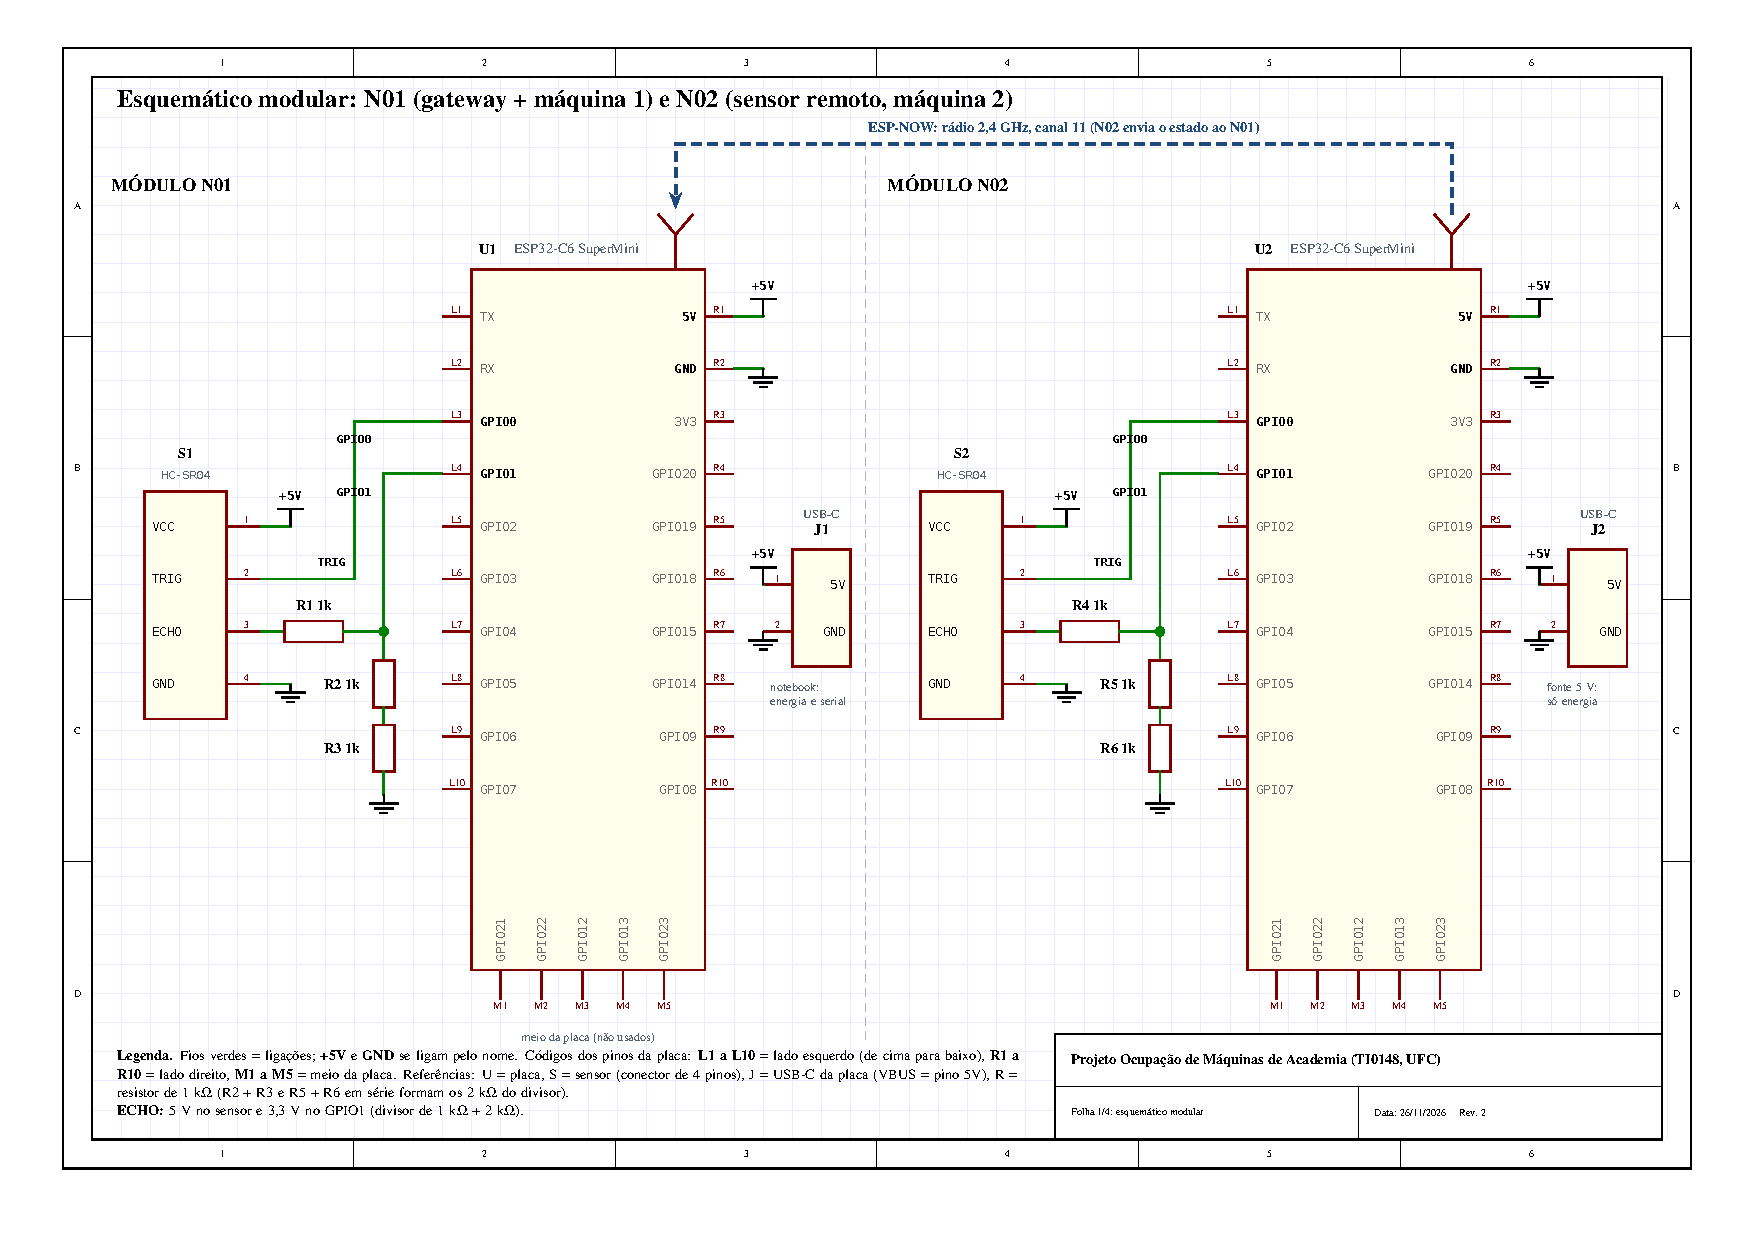
\includegraphics[page=1,trim=0.6cm 0.6cm 0.6cm 0.6cm,clip,width=0.985\textheight,angle=90]{esquematico_modular.pdf}
\end{center}
\clearpage
\restoregeometry

\subsection{Resistores do divisor}

\begin{center}
\small
\begin{tabular}{|L{2.6cm}|L{3.6cm}|L{6.4cm}|}
\hline
\textbf{Valor} & \textbf{Cores (4 faixas)} & \textbf{Onde entra} \\ \hline
1 k$\Omega$ & marrom, preto, vermelho & R1; e R2a e R2b (dois em série dão R2 = 2 k$\Omega$) \\ \hline
2,2 k$\Omega$ e 3,3 k$\Omega$ & vermelho, vermelho, vermelho \quad e \quad laranja, laranja, vermelho & alternativa: R1 = 2,2 k$\Omega$ e R2 = 3,3 k$\Omega$ (dá cerca de 3,0 V) \\ \hline
\end{tabular}
\end{center}


\begin{atencao}
\textbf{Pinos a evitar} na ESP32-C6: GPIO4 e GPIO5 (boot e JTAG), GPIO8 (boot e LED RGB), GPIO9 (boot e botão BOOT), GPIO12 e GPIO13 (USB) e GPIO15 (boot). Os nomes e a ordem dos pinos variam entre fabricantes da SuperMini: \textbf{confira a serigrafia} antes de ligar. Com o USB conectado, \textbf{não alimente o pino 5V por outra fonte} (sem diodo).
\end{atencao}

\begin{dica}
Sem o resistor de 2 k$\Omega$? Ligue \textbf{dois de 1 k$\Omega$ em série}. Se o módulo for o \textbf{HC-SR04P} (3,3 V), ligue o VCC no 3V3 e dispense o divisor.
\end{dica}

% =========================================================
\section{Roteiro passo a passo}
% =========================================================

\fase{laranja}{FASE A: MONTAR}

\passo{1}{Conferir o material}{$\approx$ 5 min}
{Leia a etiqueta do módulo ultrassônico e a serigrafia da placa.
\begin{itemize}
  \item O módulo é o \textbf{HC-SR04} (5 V)?
  \item A placa tem os pinos \textbf{GPIO0} e \textbf{GPIO1} à mostra?
\end{itemize}}
{Módulo de 5 V e os dois pinos visíveis. Se o módulo for HC-SR04P, use o VCC no 3V3 e pule o divisor. Se faltar o GPIO0 ou o GPIO1, anote quais pinos vai usar e troque no passo 4.}
{Etiqueta do módulo e serigrafia da placa.}

\passo{2}{Montar e testar o divisor de tensão}{$\approx$ 15 min}
{Com a placa \textbf{desligada do USB}, monte R1 (1 k$\Omega$) em série com R2 (dois de 1 k$\Omega$ em série). Meça cada resistência. Depois ligue a ponta livre de R1 ao 5V da placa e a ponta de R2 ao GND, conecte o USB e meça a tensão no ponto entre R1 e R2. \textbf{Desligue o USB} ao terminar.}
{R1 $\approx$ 1 k$\Omega$ e R2 $\approx$ 2 k$\Omega$. Tensão no ponto entre os dois: \textbf{3,2 a 3,4 V} (com 2,2 k$\Omega$ e 3,3 k$\Omega$: cerca de 3,0 V).}
{Multímetro, primeiro em ohms e depois em volts de corrente contínua.}

\passo{3}{Ligar os fios conforme o esquema}{$\approx$ 20 min}
{Com a placa fora do USB, ligue VCC ao 5V, GND ao GND, TRIG ao GPIO0 e ECHO ao R1, com a junção de R1 e R2 no GPIO1 (Figura~1). Peça a outra pessoa para \textbf{conferir fio por fio}. Repita na segunda placa.}
{Nenhum fio do ECHO vai direto ao GPIO. 5V e GND não estão trocados. As duas montagens são iguais.}
{Figura 1 deste roteiro e Caderno de Montagem (páginas 2 e 3).}

\fase{azul}{FASE B: PROGRAMAR}

\passo{4}{Ajustar o firmware}{$\approx$ 10 min}
{Abra \cod{firmware/app/config.h} e mude \cod{CFG_USE_SENSOR} de \cod{0} para \cod{1}. Confira \cod{CFG_PIN_TRIG} igual a \cod{0} e \cod{CFG_PIN_ECHO} igual a \cod{1} (mude se o passo 1 pediu). Depois compile: entre em \cod{firmware} e rode \cod{tools/build.sh}.}
{A compilação termina sem erro e mostra o uso de flash (cerca de 74\%).}
{Terminal.}

\passo{5}{Gravar nas duas placas}{$\approx$ 10 min}
{Liste as portas com \cod{ls /dev/serial/by-id/}. Grave \textbf{uma placa por vez}, usando o caminho que contém o MAC para não trocar de placa: \cod{tools/build.sh upload CAMINHO}, com o caminho do N01 (MAC terminado em \cod{51:80}) e depois o do N02 (terminado em \cod{61:64}).}
{O \cod{upload} termina sem erro e a placa reinicia sozinha.}
{Terminal.}

\passo{6}{Ver o boot de cada placa}{$\approx$ 10 min}
{Rode \cod{python3 tools/le_serial.py -v -t 15 PORTA}. Se não aparecer nada, \textbf{aperte o botão de reset} da placa e tente de novo. Para ver o log do N02, ele precisa estar no USB do notebook, em outra porta.}
{Uma linha de boot: \logl{boot papel=gateway no=N01 ... mede=1 fonte=hcsr04 escala=1} no N01 (e \cod{papel=sensor no=N02} no outro). O campo \cod{fonte} \textbf{tem} que ser \cod{hcsr04}, nunca \cod{simulada}. Depois, uma linha por segundo: \logl{up=... dist=... filt=... estado=0}.}
{Terminal (saída do \cod{le_serial.py}).}

\fase{verde}{FASE C: MEDIR E VALIDAR}

\passo{7}{Distância com régua}{$\approx$ 15 min}
{Use um alvo plano e duro (caixa ou parede), \textbf{perpendicular} ao sensor, a \textbf{30, 60 e 100 cm}. Espere 3 s em cada ponto e anote os valores de \cod{dist} e \cod{filt}. Depois, repita sem nada na frente.}
{\cod{dist} e \cod{filt} ficam a \textbf{3 cm ou menos} da régua e estáveis. Sem alvo: \cod{dist=-1} (sem eco) ou um valor alto.}
{Linha de log \logl{up=... dist=... filt=...}.}

\passo{8}{Histerese e tempos de decisão}{$\approx$ 20 min}
{Faça em sequência: \textbf{(a)} alvo a 50 cm por mais de 5 s; \textbf{(b)} afaste para 80 cm; \textbf{(c)} afaste para mais de 90 cm por mais de 90 s.}
{\textbf{(a)} Após cerca de 5 s: \logl{estado mudou -> OCUPADA (dist=50 cm)} e o quadro \cod{N01,1,seq}. \textbf{(b)} A 80 cm o estado \textbf{não} muda. \textbf{(c)} Após cerca de 90 s: \logl{estado mudou -> LIVRE} e o quadro \cod{N01,0,seq}. Há um sinal de vida a cada 15 s.}
{Log do nó e quadros impressos na serial do N01.}

\begin{dica}
Para não esperar 90 s, use \cod{CFG_TIME_SCALE} igual a \cod{10u} apenas neste teste (o relógio da lógica roda 10 vezes mais rápido) e \textbf{volte para} \cod{1u} depois, antes do passo 9.
\end{dica}

\passo{9}{Enlace ESP-NOW entre os nós}{$\approx$ 15 min}
{Deixe o N01 no notebook e o N02 numa fonte boa, a alguns metros. Rode \cod{python3 tools/le_serial.py -t 120 -v PORTA_DO_N01} e mude o estado do N02 uma vez.}
{Quadros \cod{N02,estado,seq} a cada 15 s e na hora em que o estado muda, com linhas \logl{rx N02 rssi=...}. No resumo final: \textbf{0 perdidos por lacuna de seq} (até 1 a 2\% a cerca de 10 m com paredes) e \cod{reinicio ao abrir a porta: nao}.}
{Resumo no fim da saída do \cod{le_serial.py}.}

\fase{cinza}{FASE D: INTEGRAR}

\passo{10}{Ponte e API}{$\approx$ 10 min}
{Rode \cod{./venv/bin/python -m server.bridge --dry-run}. Em outro terminal, rode \cod{curl localhost:8000/machines} e depois \cod{curl localhost:8000/machines/2/history}.}
{A ponte mostra linhas para \cod{N01 maquina_1} e \cod{N02 maquina_2}. O \cod{/machines} devolve \textbf{2 itens} com \cod{online: true} e \cod{state} de acordo com a distância. O histórico lista as mudanças de estado.}
{Os dois terminais (ponte e \cod{curl}).}

\passo{11}{Teste do offline}{$\approx$ 10 min}
{Com a ponte rodando, tire o USB do N02 (ou desligue a fonte) e espere cerca de 60 s. Depois religue.}
{Após cerca de 60 s: linha \cod{N02 maquina_2: ..., OFFLINE} e \cod{online: false} no \cod{/machines}. Ao religar, assim que chegar um quadro, volta \cod{online: true}.}
{Terminal da ponte e \cod{curl localhost:8000/machines}.}

\passo{12}{Gravar no Mongo (se houver chave e IP liberado)}{$\approx$ 10 min}
{Rode \cod{./venv/bin/python -m server.bridge} (sem \cod{--dry-run}) e mude o estado de uma máquina.}
{Nenhuma linha \cod{erro ao gravar ... no Mongo}. No Atlas: a coleção \cod{nodes} com 2 documentos (\cod{node} 1 e 2) e a \cod{telemetry} com uma linha por mudança de estado.}
{Atlas (Compass ou o site), coleções \cod{nodes} e \cod{telemetry}.}

\passo{13}{Registrar e guardar}{$\approx$ 10 min}
{Tire fotos da montagem, salve os prints dos logs e preencha a Seção~\ref{sec:registro}. Só depois, faça o commit do \cod{config.h} (\cod{CFG_USE_SENSOR} igual a \cod{1}) \textbf{numa branch}, nunca na \cod{main}.}
{Evidências para o relatório e para o card do Trello.}
{Fotos, tabela de registro e terminal.}

% =========================================================
\section{Critérios de aceite}
% =========================================================

\begin{itemize}[label={}]
  \item \caixa\enspace Leitura de distância a 3 cm ou menos da régua em 30, 60 e 100 cm, \textbf{nas duas placas}.
  \item \caixa\enspace Estado \textbf{ocupada} após mais de 5 s a 70 cm ou menos; \textbf{livre} após mais de 90 s a 90 cm ou mais; entre 70 e 90 cm o estado não muda.
  \item \caixa\enspace N02 chega ao N01 sem perda relevante em 2 minutos de teste.
  \item \caixa\enspace A API mostra \textbf{2 máquinas} e marca offline em cerca de 60 s ao desligar uma.
  \item \caixa\enspace (Se houver banco) \cod{nodes} e \cod{telemetry} recebem os dados.
\end{itemize}

% =========================================================
\section{Se der errado}\label{sec:erros}
% =========================================================

\begin{longtable}{|L{3.7cm}|L{5.0cm}|L{5.4cm}|}
\hline
\textbf{Sintoma} & \textbf{Causa provável} & \textbf{O que fazer} \\ \hline
\endhead
\cod{dist=-1} sempre & TRIG e ECHO trocados; sensor sem 5V; ECHO não chega ao GPIO1; alvo longe, inclinado ou macio (roupa absorve) & Conferir fios e medir 5V no VCC; usar alvo plano e duro a 30--60 cm \\ \hline
Leitura salta muito & Alvo inclinado ou irregular; jumper solto & Alvo perpendicular; reapertar os jumpers \\ \hline
Placa reinicia ou some & Fonte ou cabo ruim (queda de tensão) & Trocar fonte e cabo; usar fonte de bancada \\ \hline
Nada na serial depois de plugar & O gateway ficou mudo até um reset (visto em 25/11, causa desconhecida) & Apertar o reset do N01 e abrir a porta de novo \\ \hline
Placa não aparece em \cod{/dev/ttyACM*} & Cabo só de carga & Trocar por cabo de dados \\ \hline
Boot mostra \cod{MAC desconhecido} & Placa trocada & Atualizar o MAC em \cod{config.h} \\ \hline
N02 não aparece no N01 & Canal ou MAC errado; N02 sem energia; distância grande & Conferir \cod{canal=11} nos dois boots; aproximar; usar fonte boa \\ \hline
Muitos quadros perdidos no passo 9 & Interferência de Wi-Fi no canal 11 (já variou nos testes de casa) & Trocar \cod{CFG_CHANNEL} (1, 6 ou 11) em \cod{config.h} e regravar \textbf{as duas} placas com o mesmo canal \\ \hline
Porta ocupada ou \cod{Permission denied} & Outro programa lendo a mesma serial & Fechar o \cod{le_serial.py} ou a ponte antes de abrir outro \\ \hline
Ponte sem quadros & Porta errada & Usar \cod{--porta} com o caminho do N01 em \cod{/dev/serial/by-id/} \\ \hline
\end{longtable}

% =========================================================
\clearpage
\section{Registro dos resultados}\label{sec:registro}
% =========================================================

\renewcommand{\arraystretch}{1.7}
\begin{longtable}{|L{1.0cm}|L{3.2cm}|L{2.0cm}|L{2.0cm}|L{1.9cm}|L{3.2cm}|}
\hline
\textbf{\#} & \textbf{Medida} & \textbf{N01} \cod{filt} & \textbf{N02} \cod{filt} & \textbf{Estado} & \textbf{Observação} \\ \hline
\endhead
1 & Régua: 30 cm & & & & \\ \hline
2 & Régua: 60 cm & & & & \\ \hline
3 & Régua: 100 cm & & & & \\ \hline
4 & 50 cm (mais de 5 s) & & & & ocupada em \_\_\_ s \\ \hline
5 & 80 cm (zona morta) & & & & \\ \hline
6 & Mais de 90 cm (mais de 90 s) & & & & livre em \_\_\_ s \\ \hline
\end{longtable}
\renewcommand{\arraystretch}{1}

\medskip
\noindent\textbf{Enlace N02 para N01:} distância \rule{1.5cm}{0.3pt} m \quad quadros \rule{1.5cm}{0.3pt} \quad perdidos \rule{1.5cm}{0.3pt} \quad RSSI \rule{1.5cm}{0.3pt} dBm\par\medskip
\noindent\textbf{Offline:} desligado às \rule{1.8cm}{0.3pt} \quad marcado offline às \rule{1.8cm}{0.3pt} \quad (esperado: cerca de 60 s depois)\par

\end{document}
